%%%%%%%%%%%%%%%%%%%%%%% file template.tex %%%%%%%%%%%%%%%%%%%%%%%%%
%
% This is a general template file for the LaTeX package SVJour3
% for Springer journals.          Springer Heidelberg 2014/09/25
%
% Copy it to a new file with a new name and use it as the basis
% for your article. Delete % signs as needed.
%
% This template includes a few options for different layouts and
% content for various journals. Please consult a previous issue of
% your journal as needed.
%
%%%%%%%%%%%%%%%%%%%%%%%%%%%%%%%%%%%%%%%%%%%%%%%%%%%%%%%%%%%%%%%%%%%
% First comes an example EPS file -- just ignore it and
% proceed on the \documentclass line
% your LaTeX will extract the file if required
\begin{filecontents*}{example.eps}
%!PS-Adobe-3.0 EPSF-3.0
%%BoundingBox: 19 19 221 221
%%CreationDate: Mon Sep 29 1997
%%Creator: programmed by hand (JK)
%%EndComments
%
gsave
newpath
  20 20 moveto
  20 220 lineto
  220 220 lineto
  220 20 lineto
closepath
2 setlinewidth
gsave
  .4 setgray fill
grestore
stroke
grestore
\end{filecontents*}
%
\RequirePackage{fix-cm}
%
%\documentclass{svjour3}                     % onecolumn (standard format)
%\documentclass[smallcondensed]{svjour3}     % onecolumn (ditto)
\documentclass[smallextended]{svjour3}       % onecolumn (second format)
%\documentclass[twocolumn]{svjour3}          % twocolumn
%
\smartqed  % flush right qed marks, e.g. at end of proof
%
\usepackage{amsmath}
\usepackage{graphicx}
\usepackage{lineno}
\usepackage{natbib}
\linenumbers
%
% \usepackage{mathptmx}      % use Times fonts if available on your TeX system
%
% insert here the call for the packages your document requires
%\usepackage{epstopdf}
%\graphicspath{ {./images/results} }
\usepackage{color}
\usepackage{ctable}
%\usepackage{epsfig}
\usepackage{hyperref}
\usepackage{soul}
\usepackage{amssymb}
% etc.
%
% please place your own definitions here and don't use \def but
% \newcommand{}{}
%
% Insert the name of "your journal" with
 \journalname{Boundary-Layer Meteorology}

%
\newcommand*\patchAmsMathEnvironmentForLineno[1]{%
\expandafter\let\csname old#1\expandafter\endcsname\csname #1\endcsname
\expandafter\let\csname oldend#1\expandafter\endcsname\csname end#1\endcsname
\renewenvironment{#1}%
{\linenomath\csname old#1\endcsname}%
{\csname oldend#1\endcsname\endlinenomath}}% 
\newcommand*\patchBothAmsMathEnvironmentsForLineno[1]{%
\patchAmsMathEnvironmentForLineno{#1}%
\patchAmsMathEnvironmentForLineno{#1*}}%
\AtBeginDocument{%
\patchBothAmsMathEnvironmentsForLineno{equation}%
\patchBothAmsMathEnvironmentsForLineno{align}%
\patchBothAmsMathEnvironmentsForLineno{flalign}%
\patchBothAmsMathEnvironmentsForLineno{alignat}%
\patchBothAmsMathEnvironmentsForLineno{gather}%
\patchBothAmsMathEnvironmentsForLineno{multline}%
}


% ---------------------------------------------------------------------------------------------------------------------------------
% ---------------------------------------------------------------------------------------------------------------------------------
\begin{document}

\title{Exact analytic solution for slope flows with spatially varying eddy viscosity and diffusivity}

\titlerunning{Exact analytic solution for slope flows}        % if too long for running head


%\authorrunning{Short form of author list} % if too long for running head
\author{M.~G.~Giometto \and R.~Grandi\and J.~Fang \and M.B. Parlange}

\institute{ M.G. Giometto \at School of Architecture, Civil and Environmental Engineering, \'Ecole Polytechnique F\'ed\'erale de Lausanne, Lausanne, Switzerland \\
		\email{marco.giometto@epfl.ch}
		\and
		Riccardo Grandi \at Mathematics Institute for Geometry and Applications, \'Ecole Polytechnique F\'ed\'erale de Lausanne, Lausanne, Switzerland \\
		 \and 
		 J. Fang \at School of Architecture, Civil and Environmental Engineering, \'Ecole Polytechnique F\'ed\'erale de Lausanne, Lausanne, Switzerland \\
		 \and
		M.B. Parlange \at Civil Engineering, Faculty of Applied Sciences, University of British Columbia, Vancouver, BC, Canada
}

\date{Received: DD Month YEAR / Accepted: DD Month YEAR}
% The correct dates will be entered by the editor


\maketitle

% ABSTRACT
\begin{abstract}
An exact analytic solution of the steady-state Prandtl model equations is derived, valid for spatially varying eddy diffusivities (O'Briens type) and Prandtl number of unity. 
In this formulation profiles show significant variations in both phase and amplitude of minima-maxima with respect to the classic constant eddy viscosity model and the more recent, approximate, WKB solution. 
The near wall region is characterized by a relatively stronger surface inversion and velocity gradients, the low-level-jet is further displaced toward the wall, and its peak velocity strongly depends on the model parameter, suggesting a tighter coupling between dynamics and thermodynamics.
\end{abstract}


\section{Introduction}
Natural convection of turbulent stratified flows over sloping surfaces is ubiquitous in nature and engineering, and is of interest not only as a fundamental problem in itself, but also because of the important role it plays over a broad range of scales and applications. 
On a local scale, for instance, it governs local weather conditions, affecting atmospheric transport processes and dispersion of scalars such as heat and humidity \citep{Monti2002, Nylen2004b}. 
On a regional scale, it drives the development of deep-convective circulations \citep{Egger1985, Parish1998} and is responsible for intense cyclonic vorticity in the middle and upper troposphere \citep{Parish1992}.
Further, recent experimental field campaigns \citep{Chu1987, Oerlemans1993} have shown that persistent katabatic winds characterize the atmospheric boundary layer over snow-ice surfaces and glaciers, and therefore an accurate characterization of such flows is an essential component of understanding and modeling of the weather and climate.
However, the complex dynamics (e.g. occurrence of intermittency, waves, Kelvin-Helmholtz instabilities and low-level jets) and the lack of a satisfactory similarity theory for such flows \citep{Nadeau2012} pose a heavy burden in terms of computational requirements for numerical modellers; in most cases the required resolution is prohibitively costly \citep{Shapiro2004, Shapiro2004a, Fedorovich2009, Fedorovich2009d, Burkholder2011a}.
Because of this, conceptual models are still of great interest, and represent a valid tool for the characterization of such systems. 
A cornerstone in the understanding of natural convection of stratified fluid along a sloping surface is represented by the classic Prandtl analytic model \citep{Prandtl}, and its more recent extensions/generalizations to include the effects of Coriolis force \citep{Gutman1964}, external winds \citep{Lykosov_1972}, surface heterogeneity \citep{Egger1985, Shapiro2007, Oldroyd2014}.
The Prandtl model approximates the atmosphere in a Boussinesq sense and describes a steady flow over a thermally perturbed unbounded planar sloping surface that lies within a stratified environment, given by the following system of equations:
%
\begin{linenomath*}
\begin{eqnarray}
	N^2 u(z) \sin{\alpha} & = & d( K_H db/dz )/dz,
	\label{eqn1u} \\
	%
	b(z) \sin{\alpha} & = & -d( K_M du/dz )/dz,
	\label{eqn1b}
\end{eqnarray}
\end{linenomath*}
%
where $z$ denotes the normal-to-slope coordinate directions, $u$ is the downslope velocity, $b$ is buoyancy, $N$ is the buoyancy frequency characterizing the system (related to the background stratification), $\alpha$ is the slope angle and $K_M$ and $K_H$ denote the eddy viscosity and diffusivity (an eddy viscosity/diffusivity model has been used to parametrize turbulent fluxes of momentum and buoyancy).
Equations are integrated in $z \in \ [0,H]$ with boundary conditions $u(0)=0$, $u(H) = 0$, $b(0)=b_s$ and $b(H) = 0$ ($b_s > 0$ for upslope flows, whereas $b_s<0$ for downslope flows). 

The flow is assumed to be invariant in the downslope direction and the model can be used to determine its vertical structure \citep{NAPPO1987}.
Eqs. \ref{eqn1u} and \ref{eqn1b} state that downslope (upslope) convection of cold (warm) air is balanced by momentum flux divergence, and that along-slope generated buoyancy is balanced by buoyancy flux divergence; thus the model is applicable away from ridges and valleys, so that advection terms are negligible \citep{NAPPO1987}.
The Prandtl constant-K model is known to be overdissipative in the near surface regions, and therefore not able to represent the observed strong surface gradients of temperature and momentum that commonly characterize katabatic and anabatic flows \citep{Oerlemans1998, grisogono2001katabatic}. 
Simple variations in the eddy diffusivity profiles were introduced in an exact analytic solution by \citet{gutman_1983}, and more recently \citet{grisogono2001katabatic} considered general variations in the vertical structure of the eddy diffusivities, and derived  solutions based on the WKB approximation.
The WKB solution is able to account for additional dynamics while still retaining an elegant form.
However, that theory is only applicable when the model parameters $(K_M, K_H)$ vary more slowly than the solution $(u,b)$, and the validity of such a constraint for slope flows has been the subject of great debate \citep{Grisogono2002}.
In the following, we derive a closed-form solution to the Prandtl-model equations, valid for O'Brien's type \citep{O'Brien1970} eddy diffusivities and representing an exact alternative to the WKB solution -- for the chosen form of the model parameter. 


% ###################################################################
\section{The Analytic Solution}
%
We consider the one-dimensional Prandtl model equations \ref{eqn1u} and \ref{eqn1b}. Assuming $Pr=1$ (i.e. $K_M=K_H=K$) and assigning length, velocity and buoyancy scales as $L=\max{(K)}^{1/2} N^{-1/2} \sin^{-1/2}{\alpha}$, $U=b_s N^{-1}$ and $B=b_s$ Eqs. \ref{eqn1u} and \ref{eqn1b} can be reduced to:
%
\begin{linenomath*}
\begin{subequations}
\label{ode}
\begin{align}
	u^+& = d( K^+ db^+/dz^+ )/dz^+, && \mathrm{in}  \ [0,H^+]
	\label{eqn1u_norm} \\
	%
	b^+ & = -d( K^+ du^+/dz^+ )/dz^+, &&\mathrm{in}  \ [0,H^+]
	\label{eqn1b_norm}
\end{align}
\end{subequations}
\end{linenomath*}
%
respectively, where $K^+$ is a normalized eddy viscosity, $z^+=zL^{-1}$, $u^+ = uU^{-1}$, $b^+=b B^{-1}$, with boundary conditions $u^+(0)=0$, $u^+(H^+) = 0$, $b^+(0)=\pm 1$ and $b^+(H^+) = 0$.
%
Further, we introduce the following variables 
%
\begin{linenomath*}
\begin{equation}
   f_1= b^+ - i u^+ \hspace{3mm} \textrm{and} \hspace{3mm} f_2=b^+ + iu^+,
   \label{combinationVars}
\end{equation}
\end{linenomath*}
%
and upon substitution of Eqs. \ref{eqn1u_norm} and \ref{eqn1b_norm} into Eqs. \ref{combinationVars}, the system can be decoupled to obtain two (independent) complex ordinary differential equations (ODEs) for the canonical variables $f_1$ and $f_2$:
%
\begin{linenomath*}
\begin{subequations}
\label{ode_norm}
\begin{align}
	i \cdot f_1 &=  d(  K^+ df_1/dz^+ )/dz^+, && \mathrm{in}  \ [0,H^+]
	\label{ode1} \\
	i \cdot f_2 &= - d( K^+ df_2/dz^+ )/dz^+, && \mathrm{in}  \ [0,H^+]
	\label{ode2}
\end{align}
\end{subequations}
\end{linenomath*}
%
with boundary conditions $f_i(0)=\pm 1$ and $f_i(H^+) = 0$, $i=1,2$.

We assume eddy diffusivities in line with the classic O'Brien's type \citep{O'Brien1970}, viz. $K^+ = A^+ (z^++\epsilon^+)(z^+-H^+-\epsilon^+)^2$, where
$\epsilon^+$ is an additional parameter that we introduce in order to shift the zeroes of $K^+$ outside the interval of integration $[0,H^+]$.
$\epsilon^+$ can be tuned to provide the desired value of viscosity / diffusivity at the wall. 

In order to solve Eqs. \ref{ode1} and \ref{ode2}, we observe that both have the form
%
\begin{linenomath*}
\begin{equation*}
	f= \mp i \cdot d/dz^+ ( K^+ df/dz^+ ),
\end{equation*}
\end{linenomath*}
%
and therefore can be solved using the same method. First, we rewrite the equation in canonical form:
%
\begin{linenomath*}
\begin{align}
	\label{can_form}
	f''+P f'+ Qf &=0, && \mathrm{in}  \ [0,H^+]
\end{align}
\end{linenomath*}
%
where $P(z^+)=(K^+)'/K^+$ and $Q(z^+)=1/(\pm i K^+)$. Second, it is an easy computation to show that, if $f$ solves Eq. \ref{can_form} then $g(z^+):=f( (H^++2 \epsilon^+) z^+- \epsilon^+)$ solves:
%
\begin{linenomath*}
\begin{align}
	\label{can_form_sec}
	g''+\widetilde{P} g'+ \widetilde{Q} g =0, && \mathrm{in}  \ [0,1]
\end{align}
\end{linenomath*}
%
where $\widetilde{P}(z^+)=\gamma'(z^+)/\gamma(z^+)$ and $\widetilde{Q}(z^+)=1/(\pm i \cdot A^+ \cdot (H^++2\epsilon^+) \gamma(z^+))$, with $\gamma(z^+)=z^+(z^+-1)^2$.
Eqn. \ref{can_form_sec} is a second order ODE with three regular singular points at $z^+ = 0,1$ and $\infty$, as in \citet{Morse1954a}. 
This special case is known as the \emph{equation of Papperitz} and its general solution is:
%
%\begin{widetext}
\begin{linenomath*}
\begin{equation}
	g(z^+) = \alpha (1-z^+)^\mu \ _2F_1 (\mu, 1- \mu', 1+\mu-\mu', 1-z^+)
	+\beta (1-z^+)^{\mu'} \ _2F_1 (\mu', 1- \mu, 1+\mu'-\mu, 1-z^+),
	\label{gen_sol_g}
\end{equation}
\end{linenomath*}
%\end{widetext}
%
where $\ _2F_1$ are \emph{Gaussian hypergeometric functions} and $\mu$, $\mu'$ are the solutions to the degree two equation
%
\begin{linenomath*}
\begin{equation*}
	x^2+x+1/(\pm i A^+(H^++2 \epsilon^+))=0,
\end{equation*}
\end{linenomath*}
%
depending on which of Eqs. \ref{can_form_sec} we are solving.
Note that the general solution to Eq. \ref{can_form_sec} is also often written using the \emph{Riemann symbol}:
%
\begin{linenomath*}
\begin{equation*}
\left \{
\begin{array}{cccc}
0 & 1 & \infty &  \\
\lambda & \mu & \nu & z^+\\
\lambda' & \mu' & \nu' & \\
\end{array}
\right \}
\end{equation*}
\end{linenomath*}
%
where, in this case, $\mu$ and $\mu'$ are as above, $\lambda=\lambda'=0$ and $\nu=0$, $\nu'=2$.
%
To retrieve the general solution to Eq. \ref{can_form} it is sufficient to substitute $(z^++\epsilon^+)/(H^+ +2 \epsilon^+)$ in place of $z^+$ in Eq. \ref{gen_sol_g}.
As the integration constants $\alpha$ and $\beta$ are specified through the imposition of boundary conditions, back-substituting $b^+ = (f_1+f_2)/2$ and $u^+ = -(f_1-f_2)/2i$ yields the solution in terms of $u^+$ and $b^+$.

% ####################################################################
\section{Examples}
%
\begin{figure}
   \begin{center}
      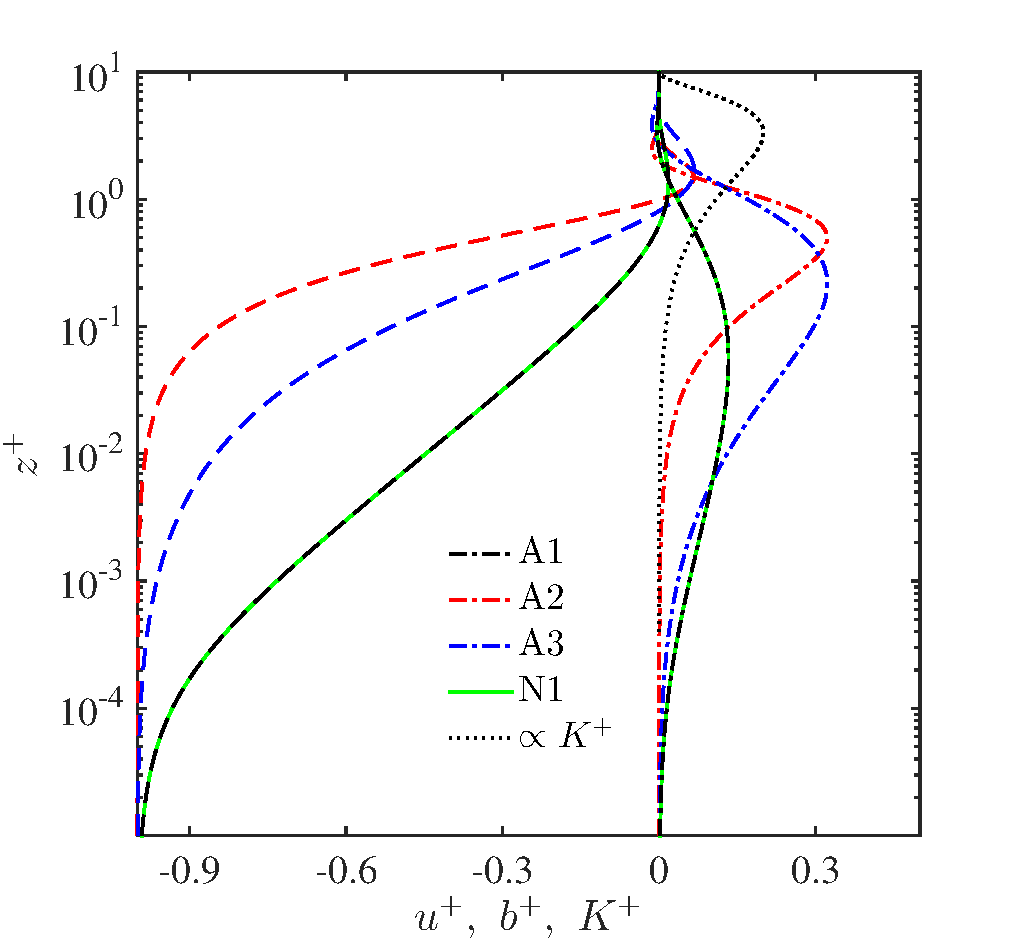
\includegraphics[width= 70.0mm]{./u-b_log}
      \caption{Comparison of the new analytic solution (A1) against the constant-$K$ (A2), the WKB (A3) and a numerical $1D$ solution (N1). Analytic profiles of normalized velocity $(u^+)$ are denoted with dot-dashed lines whereas analytic profiles of normalized buoyancy $(b^+)$ are denoted by dashed lines. Here $K^+ = A^+ \cdot (z^++\epsilon^+)(z^+-H^+-\epsilon^+)^2$ where $A^+=6.75 e-4$, $\epsilon^+ =1.5 \times 10^{-3}$ and $H^+ = 10$. A corresponding dimensional profile is characterized by $\max{(K)} = 0.1 \ \mathrm{m^2s^{-1}}$ and $K(z=0) = 10^{-5} \ \mathrm{m^2s^{-1}}$, in agreement with common atmospheric values.}
      \label{fig1}
   \end{center}
\end{figure}
%
\begin{figure}
    \begin{center}
    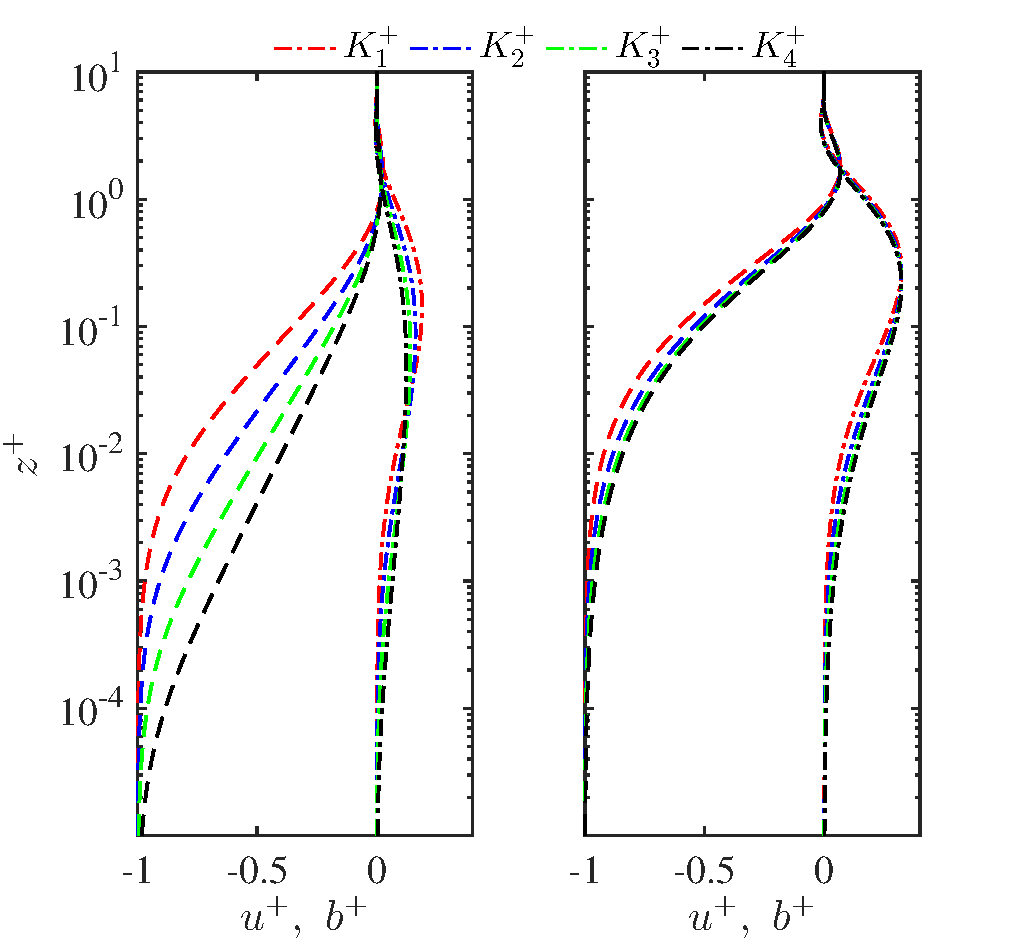
\includegraphics[width= 70.0mm]{./u-b_log_various_K}
    \caption{Sensitivity of A1 (left) and A3 (right) profiles to variations in the diffusivity coefficient $K^+$. Normalized velocity values $(u^+)$ are denoted with dot-dashed lines whereas normalized buoyancy values $(b^+)$ with dashed lines. Equations are integrated in  the interval $z^+ \in [0,10]$, which is fully shown in the plot. Here we considered $A^+=6.75 \times 10^{-4}$ and $\epsilon^+  = (7.4,1.5,0.30,0.06) \times 10^{-3}$. Under the constraint $K(z=0) = 10^{-5} \ \mathrm{m^2s^{-1}}$, the corresponding set of dimensional kynematic diffusivities satisfy $\max{(K)}=0.002,0.01,0.05,0.25 \ \mathrm{m^2s^{-1}}$.}
    \label{fig3}
    \end{center}
\end{figure}
%
In Fig. \ref{fig1} we compare the new analytic solution (A1 in the following) against the constant-$K$ (A2), the WKB (A3) and a numerical solution (N1).
The constant-$K$ value is fixed to $K^+_{\mathrm{A2}} = \max(K_{\mathrm{A1}}^+)/3$. 
Profiles for N1 are derived by solving monolithically the system of ODEs defined by Eqs. \ref{eqn1u_norm} and \ref{eqn1b_norm}, adopting a second-order accurate centered finite difference discretization with over $40,000$ collocation points and stretching the grid via a quadratic coordinate transform (at such resolution profiles are invariant to further refinements down to machine precision).
The excellent match between A1 and N1 certifies the quality of results for both methods. 
In comparison to its analytical counterparts, A1 shows a remarkably strong inversion in the near surface regions $(z^+ <1)$, suggesting overdiffusive behaviour of both A2 and A3, which are incapable of providing such strong buoyancy gradients. 
For instance, normalized surface buoyancy gradients of simulation A1 are over an order of magnitude larger than those of A2 $( (db/dz)^+_\mathrm{A1}/(db/dz)^+_\mathrm{A2} = \mathcal{O}(10)$ as $z^+ \rightarrow 0$).
Despite this, we observe a relatively good match between $u^+_\mathrm{A1}$ and $u^+_\mathrm{A3}$ in the interval $z^+ \in [0,1]$, which confirms the enhanced dissipative properties of the A3 solution, when compared against the constant-$K$ approach. 
To understand the importance of a decreasing eddy viscosity in the near surface regions, it is worth noting that $(du/dz)^+_\mathrm{A1}/(du/dz)^+_\mathrm{A2} = \mathcal{O}(10)$, whereas $(du/dz)^+_\mathrm{A1}/(du/dz)^+_\mathrm{A3}= \mathcal{O}(1)$ as $z^+ \rightarrow 0$.
Overall the new solution exhibits significant variations when compared against A2 and A3, in both amplitude and location of maxima-minima. 
For instance, both the low-level jet height and the peak normalized velocity are significantly reduced, features that are of great importance for an accurate representation of the stable boundary layer and from a parameterization perspective \citep{Mahrt1998}.
Further, from Fig. \ref{fig3}, it is clear that $\max{(u^+_\mathrm{A1})}$ now depends on the diffusive properties of the flow, i.e. $\max{(u^+_{\mathrm{A1}})} = f(K^+)$, in constrast to its analytic counterparts, which predict $\max{(u^+_\mathrm{A2})} = \max{(u^+_\mathrm{A3})} =  \sqrt{2}/2 [(e^{(\pi/4)})/\sqrt{Pr}] = 0.32$, regardless of $K^+$.
$u^+_{\mathrm{A1}}$ and $b^+_{\mathrm{A1}}$ also show a stronger dependence on the $K+$ parameter with respect to A3 profiles, in particular in the $z^+ \in [0,1]$ interval.
Overall, A1 predicts significantly reduced mass and buoyancy (horizontal) fluxes, viz. $\int_0^{H^+}{u^+}{dz^+},\int_0^{H^+}{b^+}{dz^+}$, with respect to A3.
%
% new part
%
\begin{figure}
    \begin{center}
    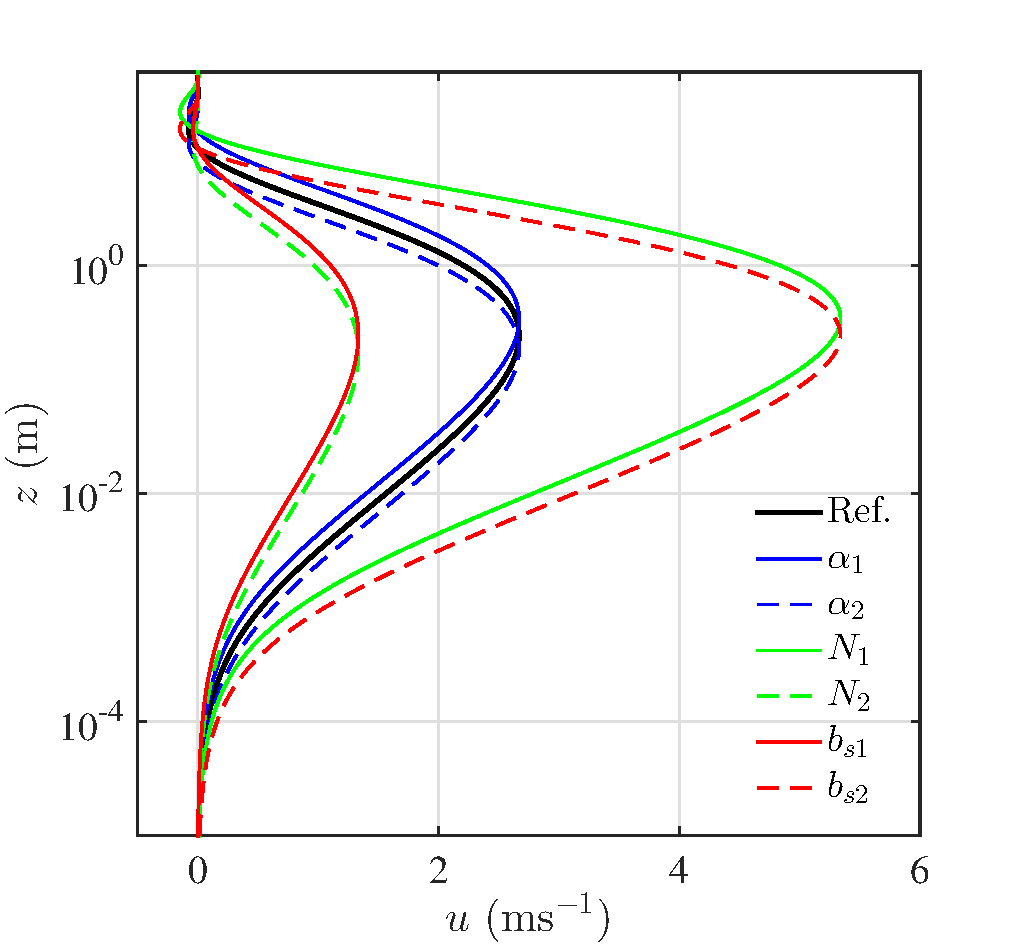
\includegraphics[width= 70.0mm]{./u_dim_alpha_N_b}
    \caption{Family of dimensional velocity profiles derived from re-dimensionalization of a reference normalized solution. The normalized solution is obtained in $z^+ \in [0,10]$ for $A^+ = 6.75 \times 10^{-4}$ and $\epsilon^+ =1.5 \times 10^{-3}$ (assuming $K(z=0) = 10^{-5}  \ \mathrm{m^2s^{-1}}$, the corresponding dimensional kynematic diffusivities satisfy $\max{(K)}=0.01 \ \mathrm{m^2s^{-1}}$). The considered set of parameters are reported in Table \ref{table}. Decreasing values of the parameters (with respect to the reference ones) are denoted with solid lines, increasing values by dashed lines.}
    \label{fig2}
    \end{center}
\end{figure}
%
\begin{table}
\caption{Set of parameters for re-normalization of the reference solution. The reference normalized solution is computed adopting $H^+ = 10, A^+ = 6.75 \times 10^{-4}, \epsilon^+ =1.5 \times 10^{-3}$.}
\label{table}
\centering
\begin{tabular}{l l l l l l l l}
\hline
 Value & Ref. & $\alpha1$ & $\alpha_2$ & $N_1$ & $N_2$ & $b_{s,1}$ & $b_{s,2}$ \\
\hline
   $\alpha \ (\mathrm{deg})$ & 30 & 15 & 60 & 30 & 30 & 30 & 30  \\
   $N \ (\mathrm{Hz})$ & 0.01 & 0.01 & 0.01 & 0.005 & 0.02 & 0.01 & 0.01 \\
   $b_s \ (\mathrm{ms^{-2}})$ & 0.30 & 0.30 & 0.30 & 0.30 & 0.30 & 0.15 & 0.60 \\
\hline
\end{tabular}
\end{table}
%
To get acquainted with the proposed normalization Fig. \ref{fig2} proposes a set of re-dimensionalized velocity profiles $u \ \mathrm{(ms^{-1})}$ from a reference normalized solution.
We propose a reference dimensional solution, characterized by $\alpha = 30 \ \mathrm{deg}, N = 0.01 \ \mathrm{Hz}$ and $b_s = 0.3  \ \mathrm{ms^{-2}}$, and consider variations in both sloping angle $\alpha$, imposed buoyancy frequency $N$ and imposed surface buoyancy $b_s$ (see Table \ref{table}).
Variations in the sloping angle $\alpha$ result in a modification of the normalization constant $L \propto \sin^{-1/2}$ which acts as a stretching of the independent variable $z$ (no effects on $\max{(u)}$). 
In particular, the steeper the angle, the smaller the characteristic scales of the flow will become.
Variations in the background stratification, viz. $N$, will modify both $L \propto N^{-1/2}$ and $U \propto N^{-1}$, yielding changes in the system, whose lengths and velocities will tend to decrease (increase) with increasing (decreasing) $N$.
Further, variations in the prescribed surface buoyancy $b_s$ will scale both buoyancy and velocity profiles accordingly, since $b(z) \propto b_s$ and $u(z) \propto b_s$.
As in both the classic Prandtl and WKB linear models, $K^+$ needs to be assigned a-priori; it is not coupled and does not feed back into the solution, which represents the main weakness of such linear approaches \citep{grisogono2001katabatic}.


% ####################################################################
\section{Conclusions}
%
We have derived a closed-form analytic solution of the Prandtl model equations, based on an ad hoc decoupling of the system and specific choice of the model parameter, resulting in a set of \textit{equations of Papperitz}, characterized by three regular singular points. 
The new solution is valid for O'Brien-type eddy diffusivities (cubic polynomials) and Prandtl number of unity. 
For the considered settings the new solution represents an improvement with respect to both the classic constant-$K$ and the more recent WKB solutions. 
New profiles show significant variations in both phase and amplitude of minima-maxima, stronger surface gradients are combined with overall reduced horizontal fluxes and the LLJ is further displaced toward the wall.
The new solution suggests a somewhat different coupling between velocity and buoyancy -- when compared against its analytical counterparts, showing a diffusivity dependent peak velocity and a remarkably strong inversion layer in the near surface location.
In addition to a theoretical insight, the proposed solution can be used to improve future stable boundary layer parameterizations when coupled with other parts of the boundary layer physics.


% ####################################################################
\section{Acknowledgements}
%
This research was primarily funded by the Swiss National Science Foundation (SNSF-200021-134892) and by the Competence Center for Environmental Sustainability (CCES-SwissEx) of the ETH domain. We are also grateful for funding from the NSERC Discovery Grant program.

%\appendix?


% BibTeX users please use one of
\bibliographystyle{spbasic}      % basic style, author-year citations
%\bibliographystyle{spmpsci}      % mathematics and physical sciences
%\bibliographystyle{spphys}       % APS-like style for physics
%\bibliography{/Users/mg/Phd/papers/bib_files/library}

\begin{thebibliography}{26}
\providecommand{\natexlab}[1]{#1}
\providecommand{\url}[1]{{#1}}
\providecommand{\urlprefix}{URL }
\expandafter\ifx\csname urlstyle\endcsname\relax
  \providecommand{\doi}[1]{DOI~\discretionary{}{}{}#1}\else
  \providecommand{\doi}{DOI~\discretionary{}{}{}\begingroup
  \urlstyle{rm}\Url}\fi
\providecommand{\eprint}[2][]{\url{#2}}

\bibitem[{Chu(1987)}]{Chu1987}
Chu PC (1987) {An instability theory of ice-air interaction for the formation
  of ice edge bands}. Journal of Geophysical Research 92(7):6966,
  \doi{10.1029/JC092iC07p06966}

\bibitem[{Egger(1985)}]{Egger1985}
Egger J (1985) {Slope Winds and the Axisymmetric Circulation over Antarctica}.
  Journal of the Atmospheric Sciences 42:1859--1867,
  \doi{10.1175/1520-0469(1985)042<1859:SWATAC>2.0.CO;2}

\bibitem[{Fedorovich and Shapiro(2009{\natexlab{a}})}]{Fedorovich2009d}
Fedorovich E, Shapiro A (2009{\natexlab{a}}) {Structure of numerically
  simulated katabatic and anabatic flows along steep slopes}. Acta Geophysica
  57(4):981--1010, \doi{10.2478/s11600-009-0027-4},
  \urlprefix\url{http://www.springerlink.com/index/10.2478/s11600-009-0027-4}

\bibitem[{Fedorovich and Shapiro(2009{\natexlab{b}})}]{Fedorovich2009}
Fedorovich E, Shapiro A (2009{\natexlab{b}}) {Turbulent natural convection
  along a vertical plate immersed in a stably stratified fluid}. Journal of
  Fluid Mechanics 636:41, \doi{10.1017/S0022112009007757}

\bibitem[{Grisogono and Oerlemans(2001)}]{grisogono2001katabatic}
Grisogono B, Oerlemans J (2001) {Katabatic Flow: Analytic Solution for
  Gradually Varying Eddy Diffusivities}. Journal of the Atmospheric Sciences
  58(21):3349--3354,
  \doi{http://dx.doi.org/10.1175/1520-0469(2001)058<3349:KFASFG>2.0.CO;2}

\bibitem[{Grisogono and Oerlemans(2002)}]{Grisogono2002}
Grisogono B, Oerlemans J (2002) {Justifying the WKB approximation in pure
  katabatic flows}. Tellus, A 54(5):453--462,
  \doi{10.1034/j.1600-0870.2002.201399.x}

\bibitem[{Gutman(1983)}]{gutman_1983}
Gutman LN (1983) {On the theory of the katabatic slope wind}. Tellus, A
  35(3):332--335, \doi{10.3402/tellusa.v35i3.11434}

\bibitem[{Gutman and Malbakhov(1964)}]{Gutman1964}
Gutman LN, Malbakhov VM (1964) {On the Theory of the Katabatic Winds of
  Antarctica}. University of Melbourne, Meteorology Department

\bibitem[{Lykosov and Gutman(1972)}]{Lykosov_1972}
Lykosov VN, Gutman LN (1972) {Turbulent boundary layer above a sloping
  inderlying surface}. Proceedings of the USSR Academy of Sciences 8:799--809,
  \urlprefix\url{papers2://publication/uuid/B2EC0692-4251-4224-8185-A1AE8D9B00E9}

\bibitem[{Mahrt(1998)}]{Mahrt1998}
Mahrt L (1998) {Stratified Atmospheric Boundary Layers and Breakdown of
  Models}. In: Theoretical and Computational Fluid Dynamics, vol~11, pp
  263--279, \doi{10.1007/s001620050093},
  \urlprefix\url{http://link.springer.com/10.1007/s001620050093}

\bibitem[{Monti et~al.(2002)Monti, Fernando, Princevac, Chan, Kowalewski, and
  Pardyjak}]{Monti2002}
Monti P, Fernando HJS, Princevac M, Chan WC, Kowalewski TA, Pardyjak ER (2002)
  {Observations of Flow and Turbulence in the Nocturnal Boundary Layer over a
  Slope}. Journal of the Atmospheric Sciences 59:2513--2534,
  \doi{10.1175/1520-0469(2002)059<2513:OOFATI>2.0.CO;2}

\bibitem[{Morse and Feshbach(1953)}]{Morse1954a}
Morse PM, Feshbach H (1953) {Methods of Theoretical Physics}. McGraw-Hill

\bibitem[{Nadeau et~al.(2013)Nadeau, Pardyjak, Higgins, and
  Parlange}]{Nadeau2012}
Nadeau DF, Pardyjak ER, Higgins CW, Parlange MB (2013) {Similarity Scaling Over
  a Steep Alpine Slope}. Boundary-Layer Meteorology 147(3):401--419,
  \doi{10.1007/s10546-012-9787-5},
  \urlprefix\url{http://link.springer.com/10.1007/s10546-012-9787-5}

\bibitem[{Nappo and Shankar(1987)}]{NAPPO1987}
Nappo CJ, Shankar RK (1987) {A model study of pure katabatic flows}. Tellus A
  39(1):61--71, \doi{10.3402/tellusa.v39i1.11740},
  \urlprefix\url{http://onlinelibrary.wiley.com/doi/10.1111/j.1600-0870.1987.tb00289.x/abstract}

\bibitem[{Nylen et~al.(2004)Nylen, {Andrew G. F.}, and Doran}]{Nylen2004b}
Nylen TH, {Andrew G F}, Doran PT (2004) {Climatology of katabatic winds in the
  McMurdo dry valleys, southern Victoria Land, Antarctica}. Journal of
  Geophysical Research 109:1--9, \doi{10.1029/2003JD003937}

\bibitem[{O'Brien(1970)}]{O'Brien1970}
O'Brien JJ (1970) {A Note on the Vertical Structure of the Eddy Exchange
  Coefficient in the Planetary Boundary Layer}. Journal of the Atmospheric
  Sciences 27:1213--1215,
  \doi{10.1175/1520-0469(1970)027<1213:ANOTVS>2.0.CO;2},
  \urlprefix\url{http://dx.doi.org/10.1175/1520-0469(1970)027<1213:ANOTVS>2.0.CO;2}

\bibitem[{Oerlemans(1998)}]{Oerlemans1998}
Oerlemans J (1998) {The atmospheric boundary layer over melting glaciers}. In:
  Clear and Cloudy Boundary Layers, vol~48, Royal Netherlands Academy of Arts
  and Sciences, pp 129--153,
  \urlprefix\url{http://igitur-archive.library.uu.nl/phys/2007-0716-203217/oerlemans\_07\_atmosphericboundarylayer.pdf}

\bibitem[{Oerlemans and Vugts(1993)}]{Oerlemans1993}
Oerlemans J, Vugts HF (1993) {A Meteorological Experiment in the Melting Zone
  of the Greenland Ice Sheet}. Bulletin of the American Meteorological Society
  74(3):355--365, \doi{10.1175/1520-0477(1993)074<0355:AMEITM>2.0.CO;2}

\bibitem[{Oldroyd et~al.(2014)Oldroyd, Katul, Pardyjak, and
  Parlange}]{Oldroyd2014}
Oldroyd HJ, Katul G, Pardyjak ER, Parlange MB (2014) {Momentum balance of
  katabatic flow on steep slopes covered with short vegetation}. Geophysical
  Research Letters 41:4761--4768, \doi{10.1002/2014GL060313}

\bibitem[{Parish(1992)}]{Parish1992}
Parish TR (1992) {On the Role of Antarctic Katabatic Winds in Forcing
  Large-Scale Tropospheric Motions}. Journal of the Atmospheric Sciences
  49:1374--1385, \doi{10.1175/1520-0469(1992)049<1374:OTROAK>2.0.CO;2}

\bibitem[{Parish and Bromwich(1998)}]{Parish1998}
Parish TR, Bromwich DH (1998) {A Case Study of Antarctic Katabatic Wind
  Interaction with Large-Scale Forcing}. Monthly Weather Review 126:199--209,
  \doi{10.1175/1520-0493(1998)126<0199:ACSOAK>2.0.CO;2}

\bibitem[{Prandtl(1942)}]{Prandtl}
Prandtl L (1942) {F\"{u}hrer durch die Str\"{o}mungslehre}. Vieweg \& Sohn,
  Braunschweig

\bibitem[{Shapiro and Fedorovich(2004{\natexlab{a}})}]{Shapiro2004a}
Shapiro A, Fedorovich E (2004{\natexlab{a}}) {Prandtl number dependence of
  unsteady natural convection along a vertical plate in a stably stratified
  fluid}. International Journal of Heat and Mass Transfer 47(22):4911--4927,
  \doi{10.1016/j.ijheatmasstransfer.2004.04.035},
  \urlprefix\url{http://linkinghub.elsevier.com/retrieve/pii/S0017931004002157}

\bibitem[{Shapiro and Fedorovich(2004{\natexlab{b}})}]{Shapiro2004}
Shapiro A, Fedorovich E (2004{\natexlab{b}}) {Unsteady convectively driven flow
  along a vertical plate immersed in a stably stratified fluid}. Journal of
  Fluid Mechanics 498:333--352, \doi{10.1017/S0022112003006803},
  \urlprefix\url{http://www.journals.cambridge.org/abstract\_S0022112003006803}

\bibitem[{Shapiro and Fedorovich(2007)}]{Shapiro2007}
Shapiro A, Fedorovich E (2007) {Katabatic flow along a differentially cooled
  sloping surface}. Journal of Fluid Mechanics 571:149,
  \doi{10.1017/S0022112006003302},
  \urlprefix\url{http://www.journals.cambridge.org/abstract\_S0022112006003302}

\bibitem[{Spalart et~al.(2011)Spalart, Strelets, and
  Garbaruk}]{Burkholder2011a}
Spalart P, Strelets M, Garbaruk A (2011) {Quality and Reliability of Large-Eddy
  Simulations II}. In: Evaluating Subgrid-ScaleModels for Large-Eddy Simulation
  of Turbulent Katabatic Flow, vol~16, pp 253--267,
  \doi{10.1007/978-94-007-0231-8},
  \urlprefix\url{http://www.springerlink.com/index/10.1007/978-94-007-0231-8}

\end{thebibliography}




\end{document}

